\chapter{Método de trabajo}
\label{chap:metodo}

\drop{A} lo largo de este capítulo se explica la forma en que se ha llevado a cabo este trabajo. Para ello, se justifica la metodología utilizada y se explican variaciones respecto a ésta.

En consecuencia, también se explica el desarrollo desde el punto de vista software y hardware, nombrando las principales tecnologías utilizadas.

\section{Introducción}

En este proyecto no es posible utilizar metodologías de gestión de proyectos como proceso unificado de desarrollo o SCRUM\cite{SCRUM}, dado que este proyecto no versa sobre el desarrollo de un producto, ni tampoco sobre el desarrollo de un software y que, en cualquier caso, será realizado por una persona.

En su lugar, se procederá a desarrollar iterativamente utilizando una heurística, en concreto, la heurística IDEAL, y a partir de los resultados obtenidos en la última fase de cada iteración, se procede a incrementar el prototipo obtenido.

\section{Heurística IDEAL}

IDEAL fue formulada por Bransford y Stein en 1984\cite{Brans93}, incluye 5 pasos de los cuales surgen el nombre de esta metodología, \textbf{I}dentificar el problema, \textbf{D}efinir y presentar el problema, \textbf{E}xplorar las estrategias viables, \textbf{A}vanzar en las estrategias y \textbf{L}ograr la solución.

La heurística IDEAL se define como iterativa e incremental, dado que repite varias veces el proceso hasta que el problema ha sido resulto por completo, e incremental puesto que cada iteración y nuevo inicio por los pasos del ciclo va incrementando las partes del proyecto a evaluar.

Para su estudio y aplicación, realmente, en vez de en cinco fases se suelen agrupar las dos primeras en una única fase\cite{Perales94}, \textit{``Identificar el problema''} y \textit{``Definir y presentar el problema''} tratan aspectos muy parecidos por lo que para evitar redundancias a la hora de realizar tareas se agrupan en una única fase.

\subsection{Identificación del problema}

En esta primera fase del ciclo a realizar, se procede a observar y analizar el problema y se determina el resultado que se debe obtener. Para esta primera fase de la heurística IDEAL, se toma como entrada la última salida del ciclo, en este caso, el prototipo obtenido en la última fase.

\begin{figure}[!h]
\centering
   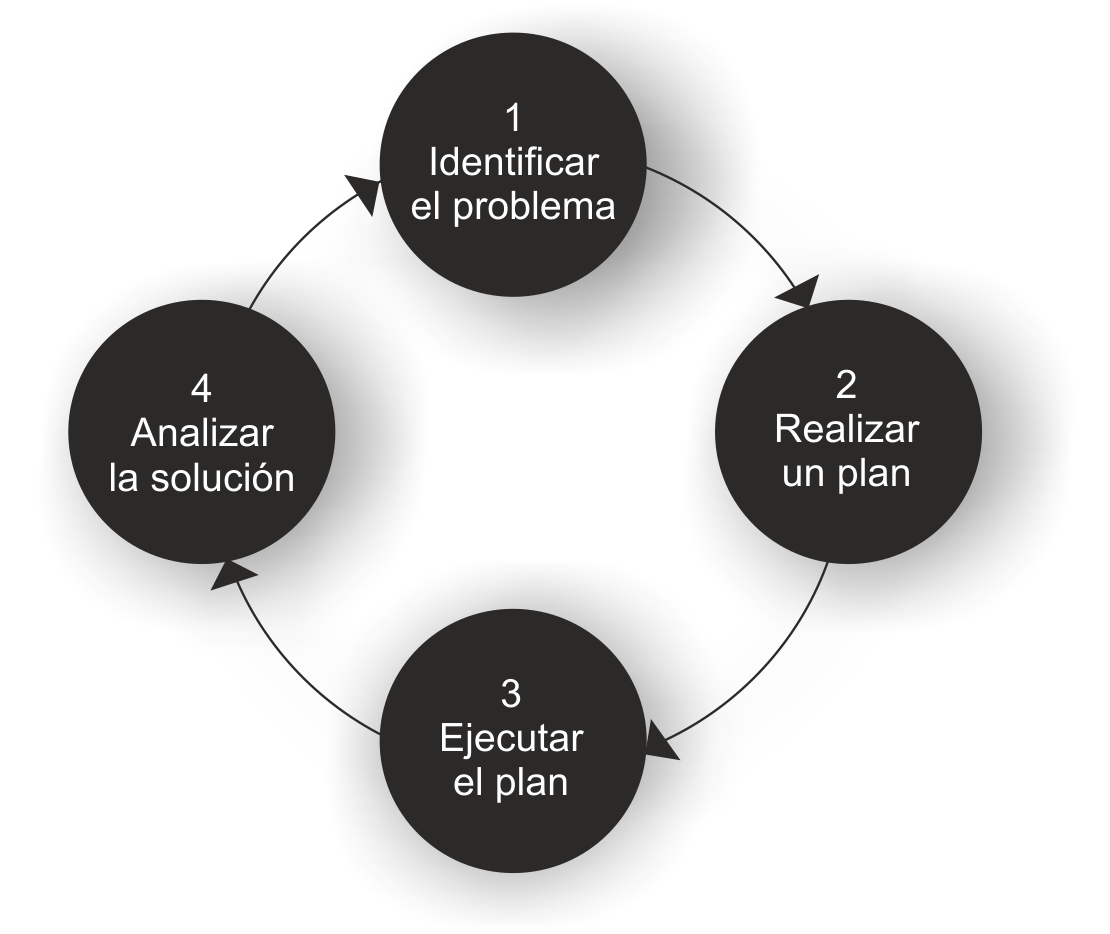
\includegraphics[width=8cm]{Ciclo_IDEAL.png}
\caption{Ciclo IDEAL}
\end{figure}

\subsection{Realización del plan}

Se determinan los pasos y operaciones a realizar para resolver el problema planteado. Por lo general, se descompone el problema en subproblemas más pequeños para facilitar la manera de resolver dicho problema. Para el desarrollo de este proyecto, tomaremos los test que debe superar la aplicación para comprobar si se han conseguido los objetivos marcados y se analizará la manera mediante la cual se deben superar dichos tests, o si se deben provocar los fallos de los tests en busca de errores.

\subsection{Ejecución del plan}

Se procede a la ejecución de cada paso del plan, siguiendo la especificación de pasos a seguir en la fase anterior ``\textit{Realización del plan}'', tras realizarse la descomposición en subproblemas más pequeños.

\subsection{Analizar la solución}

Una vez resuelto el problema identificado en la primera fase, se confirma la nueva versión del prototipo del entorno de integración continua, además, se toman técnicas de SCRUM y se realizan reuniones al final de cada iteración con \ac{Madrija} y el equipo de desarrollo para ver la evolución del prototipo, se inicia de nuevo el ciclo IDEAL desde la primera fase, tomando como entrada la salida de esta última fase, es decir, la última versión del prototipo.

\section{Aplicación del método de trabajo}
A continuación, se presenta cómo ha sido aplicada la metodología heurística IDEAL para el desarrollo de este proyecto. Cabe destacar que lo presentando en este apartado es sólo la planificación inicial de este proyecto, por lo que más adelante, en el capítulo 5, se desglosarán los pasos seguidos.

%Se estima que para la realización de este trabajo serán necesarias 5 iteraciones, la duración de cada iteración será de dos semanas.

Para la aplicación de la metodología de trabajo se va a utilizar OpenProject\cite{OpenProject} como software para gestionar el desarrollo de este proyecto.

Dentro de OpenProject, cada iteración de este desarrollo se corresponde con una versión, es decir, por cada iteración durante el desarrollo de este proyecto se realizará una nueva versión del objetivo final que se persigue. Mediante la visualización de cada versión podemos observar el número de tareas que se llevan a cabo y el estado en el que se encuentran.

\begin{figure}[!h]
\centering
   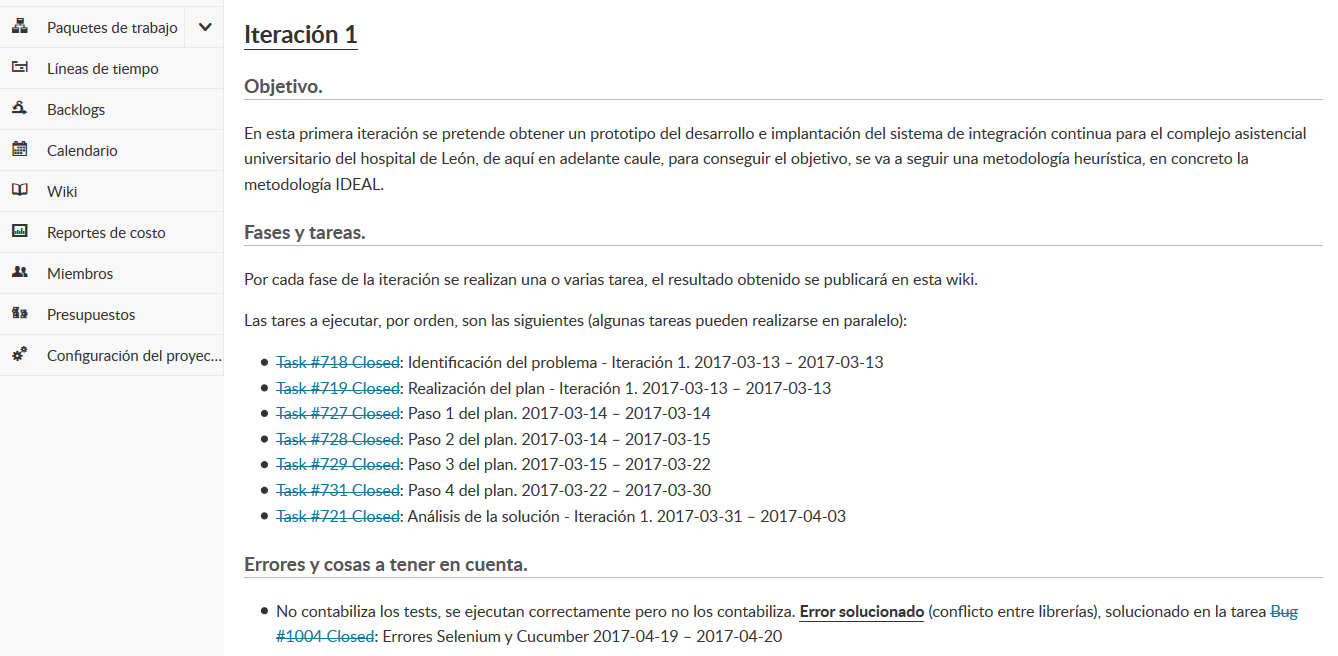
\includegraphics[width=16cm]{OpenProject1.PNG}
\caption{Imágenes de OpenProject de la iteración 1}
\end{figure}

A su vez, en las versiones de OpenProject, se desglosa en tareas el objetivo que se pretende conseguir en cada iteración, también se anotan los errores surgidos durante el desarrollo de la iteración para no cometerlos en futuras iteraciones.

Además, OpenProject consta de una wiki donde se indican las tareas que se van a realizar en cada versión, el estado de las mismas o algunos comentarios sobre, por ejemplo, errores que se han cometido para que no se realicen en el futuro.

\begin{figure}[!h]
\centering
   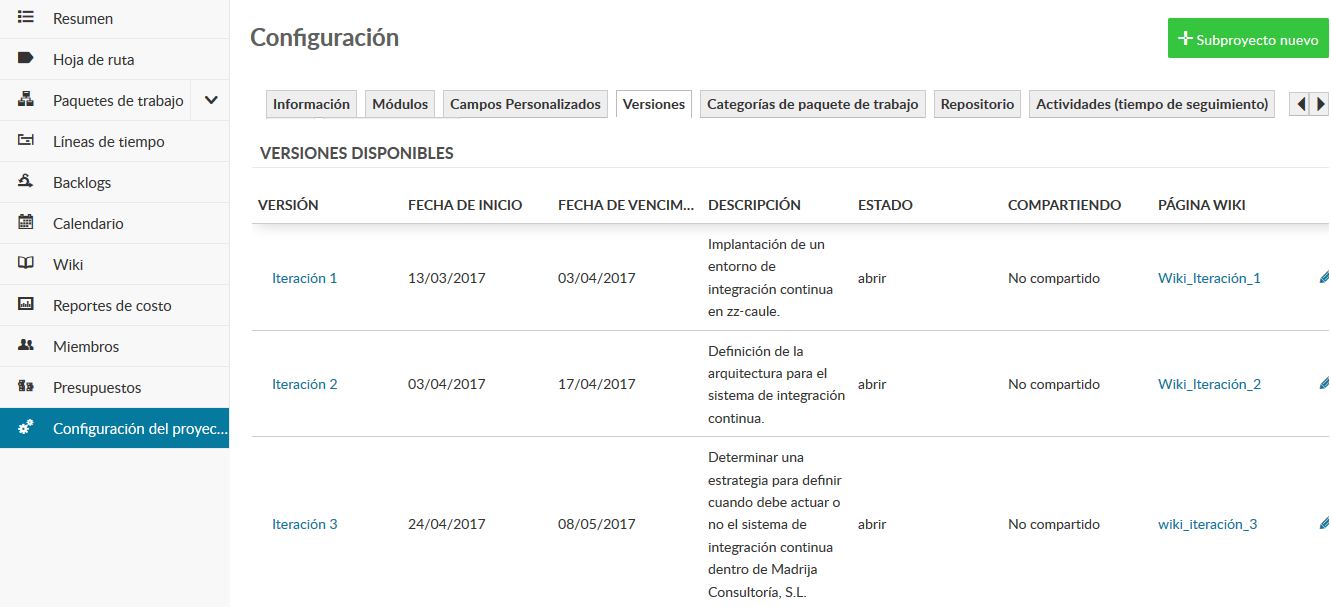
\includegraphics[width=16cm]{OpenProjectVersiones.PNG}
\caption{Algunas versiones del proyecto en OpenProject}
\end{figure}

Por lo cual, para la primera fase de la metodología heurísitca IDEAL, la fase de ``Identificación del problema'', se crea una nueva versión del proyecto con su correspondiente wiki, en dicha wiki se indica el propósito de esa versión y se crea una tarea de tipo ``\textit{Meeting}'', la cual indica que se va a realizar una reunión con \ac{Madrija} para tratar los problemas que se desean solucionar y para obtener los requisitos de esta nueva versión.

\newpage

Dado que en esta primera fase se debe realizar la captura de los requisitos, se ha optado por utilizar varias técnicas de captura de requisitos para conseguir obtener, con la mayor firmeza posible, los requisitos que se deben cumplir en cada versión de cada iteración. Se han utilizado las siguientes técnicas:
\begin{itemize}
	\item \textbf{Entrevistas\cite{toro2000metodologia}: } técnica que consiste en mantener una o más reuniones entre dos o más personas, en las que se plantean una serie de preguntas para obtener las correspondientes respuestas en el contexto de un determinado dominio de problemas.
	\item \textbf{Cuestionarios\cite{monsalve2010evolucion}: } esta técnica consiste en la elaboración de preguntas con el propósito de obtener información de los usuarios encuestados.
	\item \textbf{\textit{Brainstorming}: } es una técnica basada en reuniones en grupo cuyo objetivo es la generación de ideas en un ambiente libre de críticas o juicios.
\end{itemize}

Posteriormente, en la segunda fase del de la heurística IDEAL, se realiza otra tarea en OpenProject, en la cual se describe el plan a seguir para cumplir el objetivo marcado en el paso anterior.

Una vez finalizada la fase de ``\textit{Realización del plan}'', se crean las tareas correspondientes a cada paso a seguir del plan elaborado, no hay un número fijo de tareas, dado que cada plan de cada versión puede tener un número distinto de pasos a seguir.

\newpage

\begin{figure}[!h]
\centering
   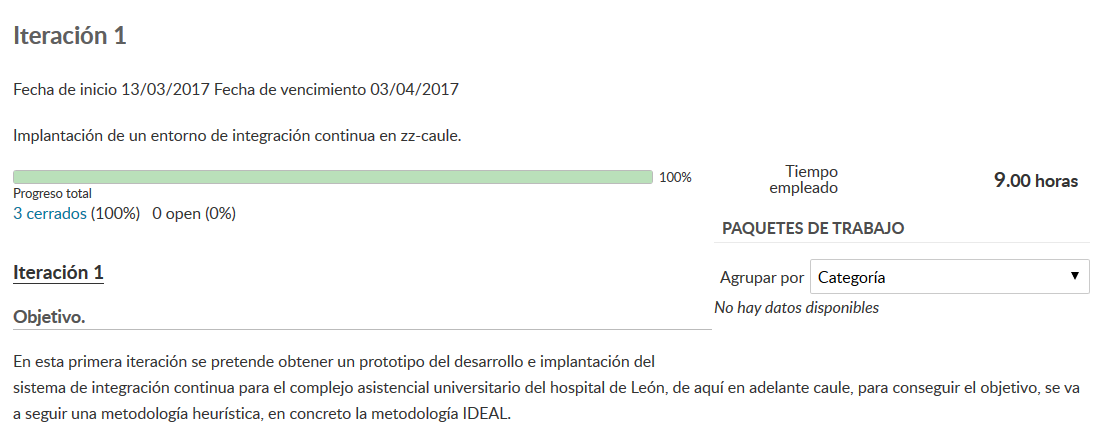
\includegraphics[width=16cm]{Parte1_Wiki_It1.PNG}
\caption{Ejemplo de la información que se muestra en la wiki de la iteración 1 (Parte 1)}
\end{figure}

Por último, se realiza una tarea llamada ``Análisis de la solución'', en la cual tras realizar todos los pasos del plan, se evaluan los resultados obtenidos así como los errores encontrados (tanto los resueltos, como los no solucionados) y se cierra esta versión.\\ \\

\begin{figure}[!h]
\centering
   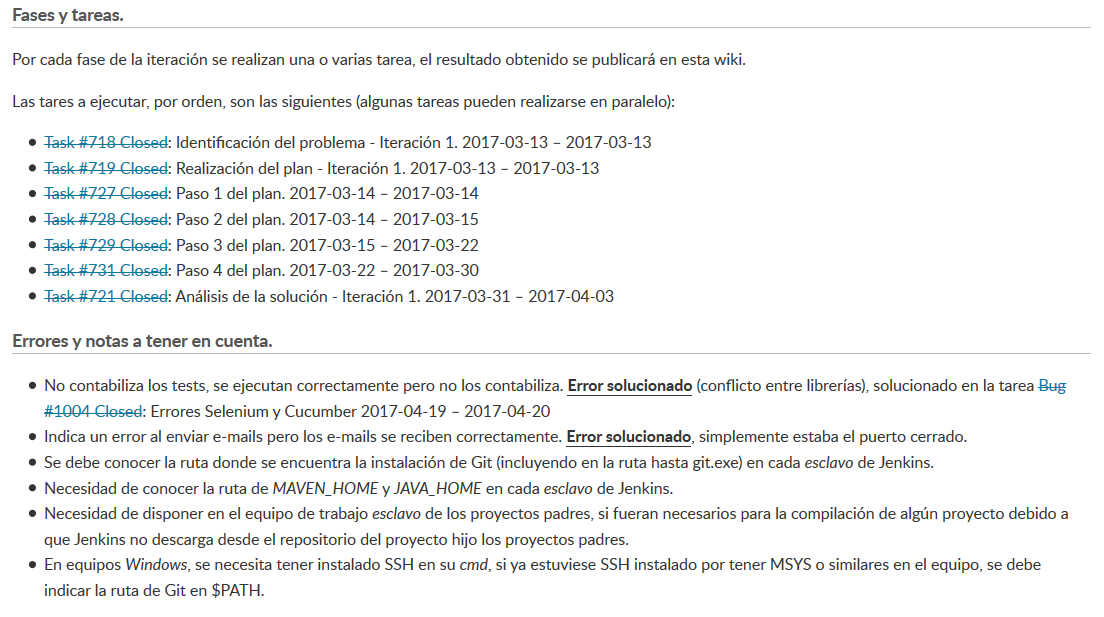
\includegraphics[width=16cm]{Parte_Wiki_It1.PNG}
\caption{Ejemplo de la información que se muestra en la wiki de la iteración 1 (Parte 2)}
\end{figure}

\newpage

\section{Planificación de las iteraciones}

Se estima que para la realización de este trabajo serán necesarias 5 iteraciones, la duración de cada iteración será de dos semanas.

\begin{center}
\rowcolors{1}{gray!25}{white}
\begin{longtable}{p{.40\textwidth} p{.60\textwidth}}
\hline \hline
  \textbf{Iteración} & \textbf{Propósito} \\
    \hline \hline
    Iteración 1. & En esta primera iteración se pretende desarrollar una prueba de concepto como prototipo del sistema de integración continua.\\
    \hline\hline
    Iteración 2. & En esta segunda iteración se pretende obtener como resultado un prototipo de una infraestructura y arquitectura para el entorno de integración continua.\\
    \hline \hline
    Iteración 3. & En la tercera iteración se pretende obtener una estrategia que active las ejecuciones del entorno de integración continua, permitiendo así obtener el mayor rendimiento y beneficio posible del mismo.\\
    \hline \hline
    Iteración 4. & En la cuarta iteración se pretende acoplar al sistema de integración continua el software ``Renombrator" que permite encontrar palabras claves que no pueden ser utilizadas para nombrar columnas en las bases de datos y cambiarlas por nombres válidos.\\
    \hline \hline
    Iteración 5. & En la quinta iteración se pretende añadir SonarQube al sistema de integración continua para que mida la calidad del código de \ac{Madrija}.\\
    \hline \hline
    \rowcolor{white}\caption{Iteraciones}
\end{longtable}
\end{center}

\newpage

\section{Marco tecnológico}
\subsection{Medios software}

Debido a que este trabajo se realiza mediante un convenio FORTE, las herramientas a utilizar son impuestas por la empresa.

\begin{itemize}
\item \textbf{Sistemas operativos}
\begin{itemize}
\item \textbf{Windows 10 Home x64: }Estación de trabajo.
\item \textbf{Ubuntu Server x64: }Servidor de la empresa.
\end{itemize}
\end{itemize}

\begin{itemize}
\item \textbf{Herramientas y tecnologías para el desarrollo software}
\begin{itemize}
\item \textbf{Jenkins: }servidor de integración continua de código abierto\cite{Jenkins}.
\end{itemize}
\begin{itemize}
\item \textbf{Java: }lenguaje de programación y una plataforma informática comercializada por Sun Microsystems\cite{Java}.
\end{itemize}
\begin{itemize}
\item \textbf{JUnit: }conjunto de bibliotecas creadas por Erich Gamma y Kent Beck que son utilizadas en programación para hacer pruebas unitarias de aplicaciones Java\cite{JUnit}.
\end{itemize}
\begin{itemize}
\item \textbf{Maven: }es una herramienta que se utiliza para construir y gestionar cualquier proyecto, y sus dependencias, basado en Java.
\end{itemize}
\begin{itemize}
\item \textbf{Eclipse: }\ac{IDE}, es una plataforma de software compuesto por un conjunto de herramientas de programación de código abierto multiplataforma para desarrollar software\cite{Eclipse}.
\end{itemize}
\begin{itemize}
\item \textbf{Selenium: }entorno de pruebas de software para aplicaciones basadas en la web\cite{Selenium}.
\end{itemize}
\begin{itemize}
\item \textbf{Cucumber: }herramienta de automatización de pruebas\cite{Cucumber} para \ac{BDD}.
\end{itemize}
\end{itemize}

\begin{figure}[!h]
\centering
   
\includegraphics[width=8cm]{Algunas_tecnologias_utilizadas.png}
\caption{Algunas tecnologías utilizadas en este desarrollo}
\end{figure}

\begin{itemize}
\item \textbf{Control de versiones}
\begin{itemize}
\item \textbf{Git:} sistema de control de versiones de código abierto\cite{Git}.
\item \textbf{GitLab:} plataforma de desarrollo colaborativo para el alojamiento de proyectos que utilizan el sistema de control de versiones Git\cite{GitLab}.
\end{itemize}
\end{itemize}

\begin{itemize}
\item \textbf{Modelado y documentación}
\begin{itemize}
\item \textbf{\LaTeX: }es un sistema de composición de textos, orientado a la creación de documentos escritos que presenten una alta calidad tipográfica\cite{LaTeX}.
\item \textbf{Inkscape: }software para edición de imágenes basado en gráficos vectoriales\cite{Inkscape}.
\end{itemize}
\end{itemize}

\begin{itemize}
\item \textbf{Herramientas para la virtualización}
\begin{itemize}
\item \textbf{Oracle VM VirtualBox: }Oracle VM VirtualBox es un software de virtualización para arquitecturas x86/amd64\cite{VirtualBox}.
\end{itemize}
\begin{itemize}
\item \textbf{Vagrant: }herramienta para la creación y configuración de entornos de desarrollo virtualizados\cite{Vagrant}.
\end{itemize}
\end{itemize}

\begin{itemize}
\item \textbf{Herramientas de bases de datos}
\begin{itemize}
\item \textbf{HSQLDB: }\textbf{H}yperthreaded \textbf{S}tructured \textbf{Q}uery \textbf{L}anguage \textbf{D}ata\textbf{B}ase, es un sistema gestor de bases de datos, libre escrito en Java\cite{HSQLDB}. 
\end{itemize}
\begin{itemize}
\item \textbf{Liquibase: }es una biblioteca independiente de bases de datos de código abierto para el seguimiento, la gestión y la aplicación de los cambios de esquema de base de datos\cite{Liquibase}.
\end{itemize}
\begin{itemize}
\item \textbf{DBeaver: }herramienta para la gestión de bases de datos\cite{DBeaver}.
\end{itemize}
\end{itemize}

\begin{itemize}
\item \textbf{Herramientas para la gestión del proyecto}
\begin{itemize}
\item \textbf{OpenProject:} software dedicado a la gestión de proyectos\cite{OpenProject}.
\item \textbf{Microsoft Project:} software dedicado a la gestión de proyectos, en especial, para diagramas de Gantt\cite{MicrosoftProject}.
\end{itemize}
\end{itemize}

\begin{itemize}
\item \textbf{Herramientas para la comunicación entre el servidor y los clientes} 
\begin{itemize}
\item \textbf{Java Web Start:} permite iniciar aplicaciones Java que se encuentran en un servidor web de aplicaciones, pero antes, comprueba que el cliente posee la última versión de la aplicación, si no la tiene, se debe actualizar la versión del cliente e inicia la comunicación. El inicio de las aplicaciones se realiza mediante enlaces a una página web o a través de enlaces de escritorio desde el cliente\cite{JavaWebStart}.
\item \textbf{SSH:} herramienta para administración remota o acceso a equipos privados a través de una puerta trasera, denominada \textit{backend}, permite manejar un equipo por completo a través de la línea de comandos\cite{SSH}.
\end{itemize}
\end{itemize}

\subsection{Medios hardware}

\begin{itemize}
\item \textbf{PC:} Ordenador portátil HP NOTEBOOK 15-r213ns con las siguientes características hardware:
\begin{itemize}
\item Procesador Intel(R) Core(TM) i7-5500U CPU @ 2.40GHz.
\item 8 GB RAM.
\item HDD 1 TB.
\end{itemize}

\item \textbf{Servidor:} HP ProLiant DL360 G7 con las siguientes características:
\begin{itemize}
\item 12 CPUs x Intel(R) Xeon(R) CPU X5650 @ 2.67 GHz.
\item 32 GHz de CPU.
\item 16 GB RAM.
\item HDD 400 GB.
\item VMWare ESXi versión 6.5.0.
\end{itemize}

\end{itemize}
